\documentclass[a4paper]{article}

\usepackage{graphicx}
\usepackage{amsmath,amssymb}
\usepackage{minted}
\usepackage{multirow}
\usepackage{float}
\usepackage{algorithm}
\usepackage{algpseudocode}
\usepackage{todonotes}
\usepackage{forest}
\usepackage{xstring}
\usepackage{xcolor}
\usepackage[most]{tcolorbox}
\usepackage{xparse}
\usepackage{natbib}
\usepackage{adjustbox}

\usetikzlibrary{graphs,graphdrawing}
\usegdlibrary{layered}

% for external graphviz
\input{/home/donkarlo/Dropbox/repo/nd_language_ai_project/src/nd_language_ai/formal/computer/programming/tex/latex/code_clips/external_graphviz.tex}

% for tags
\input{/home/donkarlo/Dropbox/repo/nd_language_ai_project/src/nd_language_ai/formal/computer/programming/tex/latex/part/control_sequence/kind/semtag/semtag.tex}

% for links
\input{/home/donkarlo/Dropbox/repo/nd_language_ai_project/src/nd_language_ai/formal/computer/programming/tex/latex/code_clips/seehere.tex}

% for nested lists and sections
\input{/home/donkarlo/Dropbox/repo/nd_language_ai_project/src/nd_language_ai/formal/computer/programming/tex/latex/code_clips/deep_structure.tex}

\title{Autonomous navigation}
\date{}
\author{Mohammad Rahmani}

\begin{document}
   \maketitle
   \label{autonomous_navigation}
   Autonomous navigation is based on minimizing the anomaly signal.

   \section{Definitions}
      \subsection{Perception--action cycle}
         \seeherefooter{/nd_robotic_ai_learning_project/src/robot/part/mind/cognition/part/object_level/process/part/thinking/planning/perception_action_cycle.tex}
         \cite{fuster-2004-upper-processing-stages-of-the-perception-action-cycle} argues that perception and action form a continuous functional cycle rather than separate processing stages. Higher cortical areas integrate perceptual information with goals, memory, and behavioral context to guide actions. The consequences of actions generate new sensory information, thereby closing and continuously updating the perception--action cycle.

         \cite{khilkevich-2024-brain-wide-dynamics-linking-sensation-to-action-during-decision-making}  shows that, after learning, sensory evidence is integrated across many brain regions in mice rather than in a single specialized area. The integrated evidence drives movement-preparatory activity, and this preparatory activity is distinct from the neural dynamics that execute the movement. Overall, the study argues that the transformation from sensation to action is brain-wide, parallel, and shaped by learning.
      \subsection{Planning}
         \seeherefooter{/nd_robotic_ai_learning_project/src/robot/part/mind/cognition/part/object_level/process/part/thinking/planning/planning.tex}
         \cite{mattar-2026-planning-in-the-brain-its-not-what-you-think-it-is}
         Planning is the cognitive process of using internal simulations of possible future actions and states to guide behavior and learning.
         
      

      \subsection{Flight controller unit (FCU)}
         A flight controller unit (FCU) refers to hardware, such as Pixhawk, used to manage the relationship among sensors, actuators, and the CPU.

      \subsection{Autopilot}
         \seeherefooter{/nd_robotic_ai_learning_project/src/robot/part/body/part/nervous_system/platform/flight_controller/autopilot/kind/px4/px4.tex}
         An autopilot is software that uses the shared data flowing through the system to generate the appropriate control signals so that the agent can achieve its next goal.

      \subsection{Controller}
      \seeherefooter{/nd_robotic_ai_learning_project/src/control_theory/controller/controller.tex}
       A controller is the part of a control system that determines the control input applied to a plant or process in order to influence its behavior toward a desired objective \cite{astrom-2008-feedback-systems-an-introduction-for-scientists-and-engineers}.
         \begin{figure}[H]
            \centering
            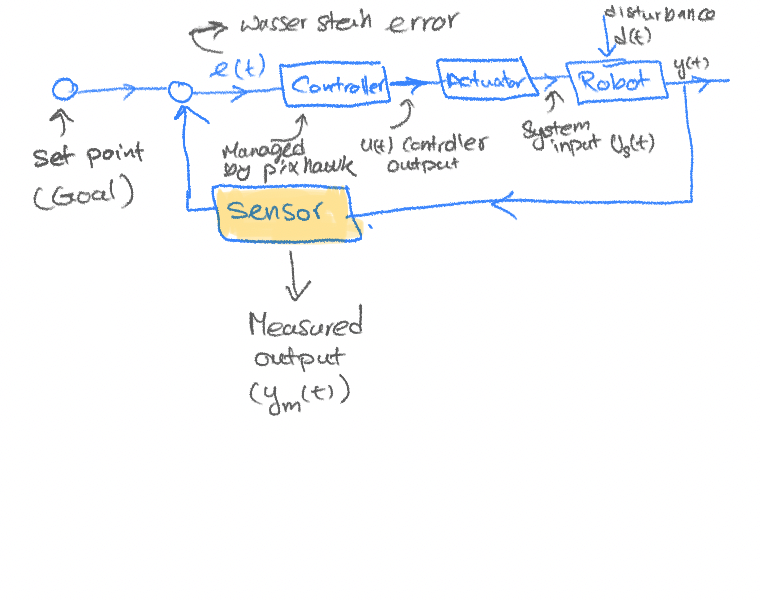
\includegraphics[width=0.9\textwidth]{controller.png}
         \end{figure}
         
         \subsubsection{P controller}
            \seeherefooter{/nd_robotic_ai_learning_project/src/control_theory/kind/proportional_controller/proportional_controller.tex}
            A proportional controller is a feedback controller whose control output is proportional to the current control error \cite{astrom-2008-feedback-systems-an-introduction-for-scientists-and-engineers}.

         \subsubsection{PID controller}
            \seeherefooter{/nd_robotic_ai_learning_project/src/control_theory/kind/proportional_integral_derivative_controller/proportional_integral_derivative_controller.tex}
            A proportional--integral--derivative (PID) controller is a feedback controller that combines the present control error, the accumulated past error, and the rate of change of the error to generate a corrective control input \cite{astrom-2008-feedback-systems-an-introduction-for-scientists-and-engineers}.
            
         \subsection{Cascade controller}
         Controllers can also be connected in a cascade. In cascade control, the output of an outer controller becomes the setpoint of an inner controller \cite{lee-1998-pid-controller-tuning-for-cascade-control-systems}. For example, an outer proportional position controller can generate a desired velocity that is tracked by an inner PID velocity controller.
   \section{Solution}

      \subsection{Data flow}
         \begin{figure}[H]
            \centering
            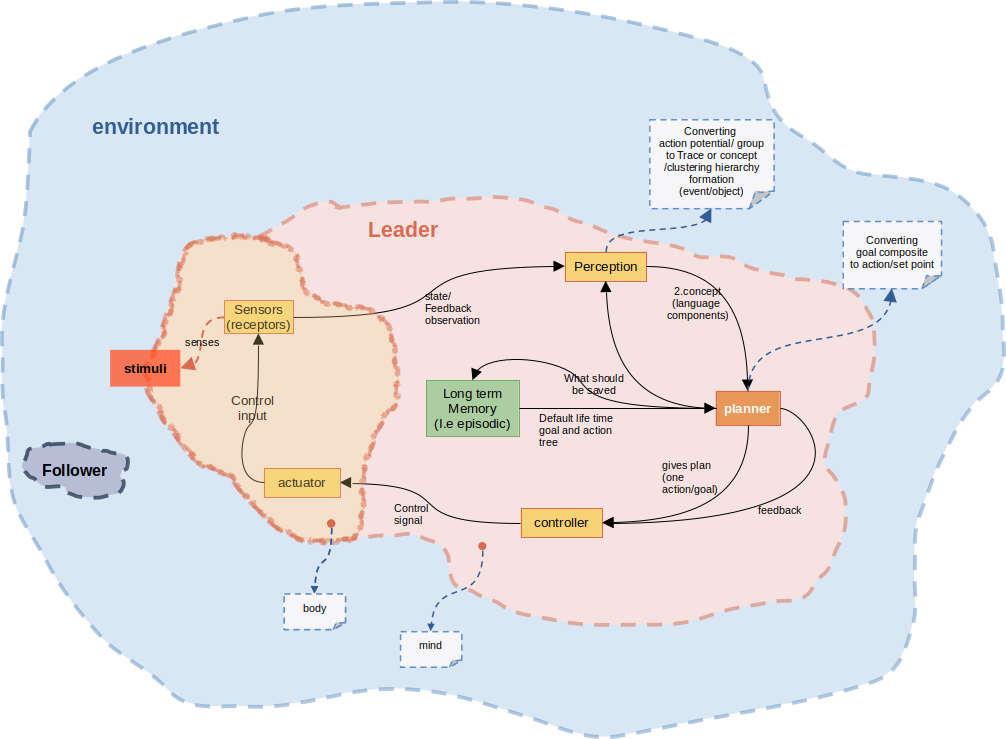
\includegraphics[width=0.9\textwidth]{data_flow.png}
         \end{figure}
         At each abstraction level during training, the system learns which actions are associated with particular exteroceptive situations. These learned actions, together with a controller, can be used to reduce the Wasserstein distance between the desired state and the current state. The system can select the appropriate second derivative to provide to the autopilot for execution at any level of the hierarchy, from the top (most abstract) when the distance is large to the bottom when the distance is small.

         For example, in the scenarios presented in this research, at an intermediate abstraction level the system has learned the commands go north, go west, go east, and go south. This is the learned language of one robot.



         \begin{figure}[H]
            \centering
            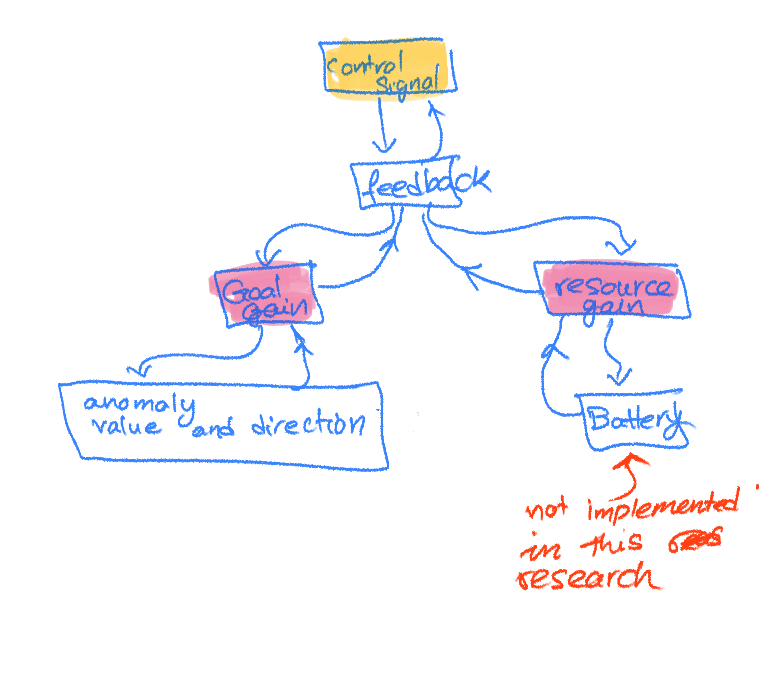
\includegraphics[width=0.9\textwidth]{feedback.png}
         \end{figure}

      \subsection{Control}

         \begin{figure}[H]
            \centering
            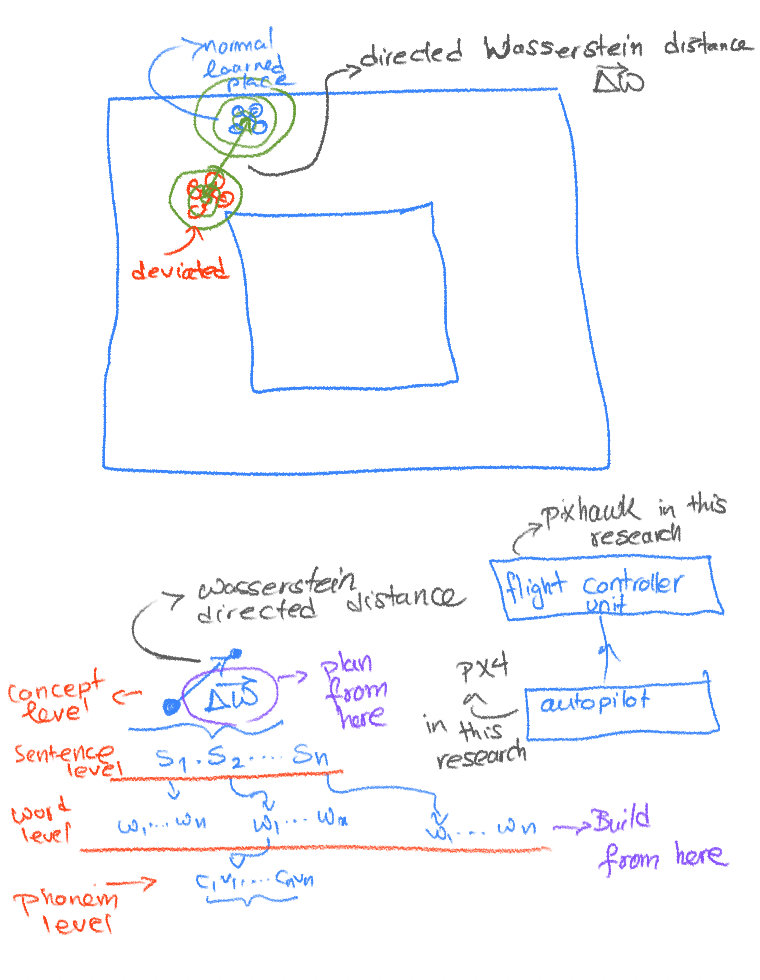
\includegraphics[width=0.9\textwidth]{autonomous_using_cost_function.png}
         \end{figure}

      \subsection{Plan}
         \seeherefooter{/nd_robotic_ai_learning_project/src/robot/part/mind/plan/plan.tex}

         In this research, a plan is conceptualized as a goal tree. Each goal is represented as a vector, whether it concerns reaching a pose (the term used in this research for both position and orientation) or a high-level goal such as keeping homeostasis or allostasis below a threshold.

         In this research, homeostasis or allostasis is considered to remain below a threshold when the Wasserstein distance between the prediction and the observation is continuously kept below that threshold.

         In this research, planning proceeds from top to bottom; that is, a group of sentences first forms the concept of moving around the perimeter of a corridor.
         \begin{figure}[H]
            \centering
            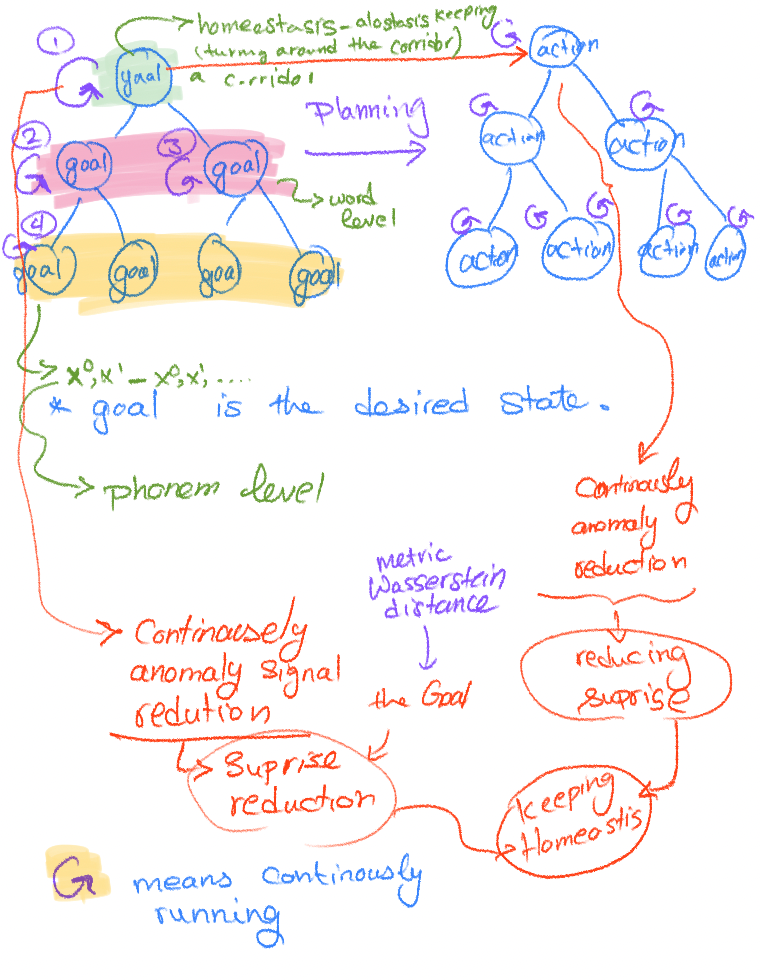
\includegraphics[width=0.9\textwidth]{plan_as_tree.png}
         \end{figure}

      \subsection{Planning}


         In this research, planning is based on decomposing the anomaly vector at each level into anomaly vectors at lower levels.

         \begin{figure}[H]
            \centering
            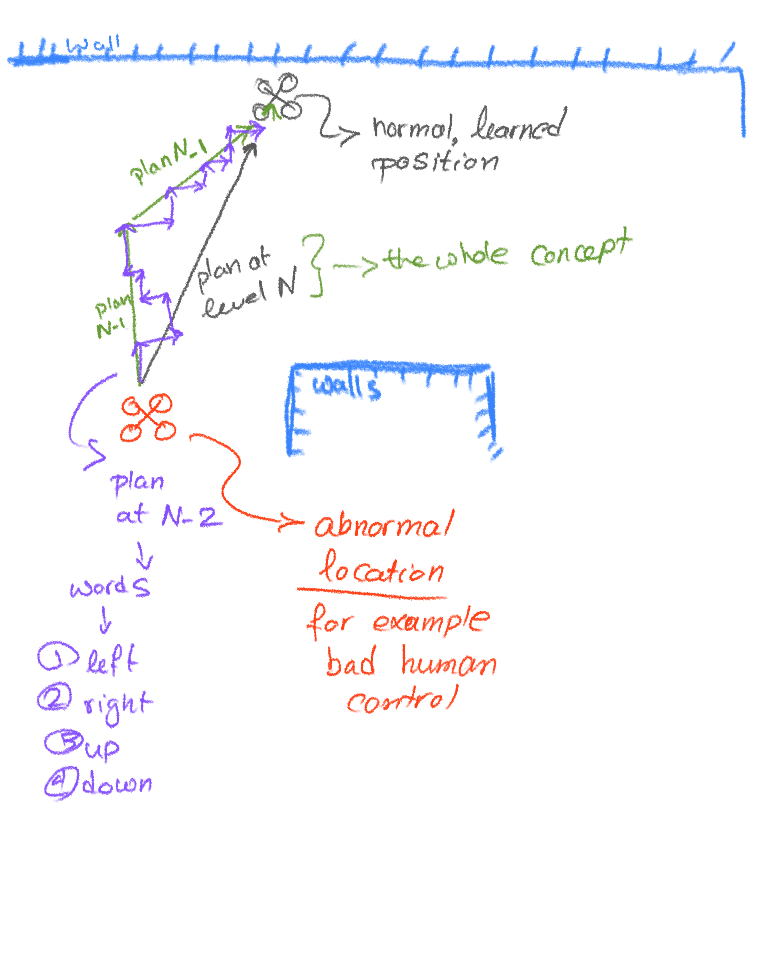
\includegraphics[width=0.9\textwidth]{planning_by_breaking.png}
         \end{figure}


      \subsection{Proposed model}
         \begin{figure}[H]
            \centering
            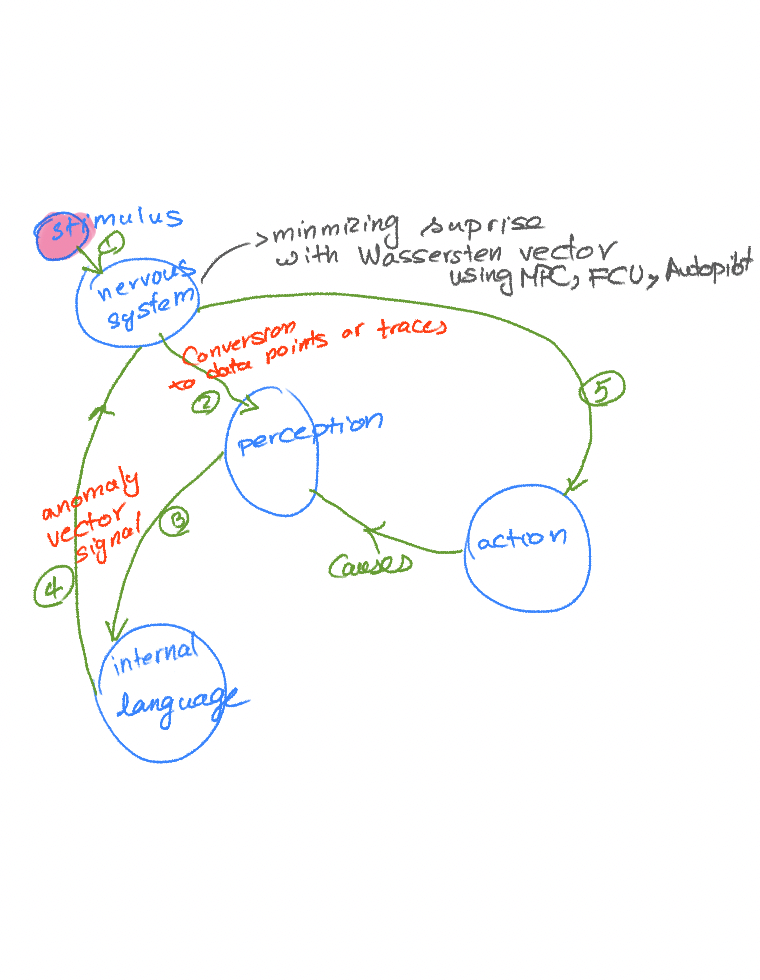
\includegraphics[width=0.9\textwidth]{language_perception_action.png}
         \end{figure}

      \subsection{Surprise reduction through directed Wasserstein discrepancy and cascaded P/PID control}

         Gaussian Wasserstein distance is used in this research as the discrepancy measure between the estimated current state distribution and the preferred state distribution. The resulting directed Wasserstein discrepancy provides both the magnitude and the direction of the mismatch between the current and preferred states.

         From the perspective of active inference, the system reduces surprise by reducing the discrepancy between predicted or estimated sensory states and preferred states \cite{friston-2010-the-free-energy-principle-a-unified-brain-theory}. In this research, this discrepancy is represented by a directed Wasserstein vector and is used as the error signal that drives action selection and low-level control.

         The directed Wasserstein discrepancy is defined as
         \[
         \mathbf{w}_k
         =
         W_2
         \left(
         p(x_k),
         p(x_k^{\mathrm{ref}})
         \right)
         \frac{
         \mu_k^{\mathrm{ref}}-\mu_k
         }{
         \left\|
         \mu_k^{\mathrm{ref}}-\mu_k
         \right\|
         },
         \]
         where \(p(x_k)\) is the estimated current state distribution and \(p(x_k^{\mathrm{ref}})\) is the preferred state distribution.

         For Gaussian state distributions,
         \[
         \begin{aligned}
            W_2^2
            \left(
            \mathcal{N}(\mu_k,\Sigma_k),
            \mathcal{N}(\mu_k^{\mathrm{ref}},\Sigma_k^{\mathrm{ref}})
            \right)
            &=
            \left\|
            \mu_k-\mu_k^{\mathrm{ref}}
            \right\|_2^2
            \\
            &\quad+
            \operatorname{Tr}
            \left(
            \Sigma_k+\Sigma_k^{\mathrm{ref}}
            -
            2
            \left(
            (\Sigma_k^{\mathrm{ref}})^{1/2}
            \Sigma_k
            (\Sigma_k^{\mathrm{ref}})^{1/2}
            \right)^{1/2}
            \right).
         \end{aligned}
         \]

         The magnitude of \(\mathbf{w}_k\) represents the Wasserstein discrepancy, while its direction points from the current state distribution toward the preferred state distribution.

         At abstract cognitive levels, this discrepancy is interpreted as a mismatch between the current and desired states. At the physical control level, the discrepancy is executed through a cascaded P/PID controller structure.

         \begin{figure}[H]
            \centering
            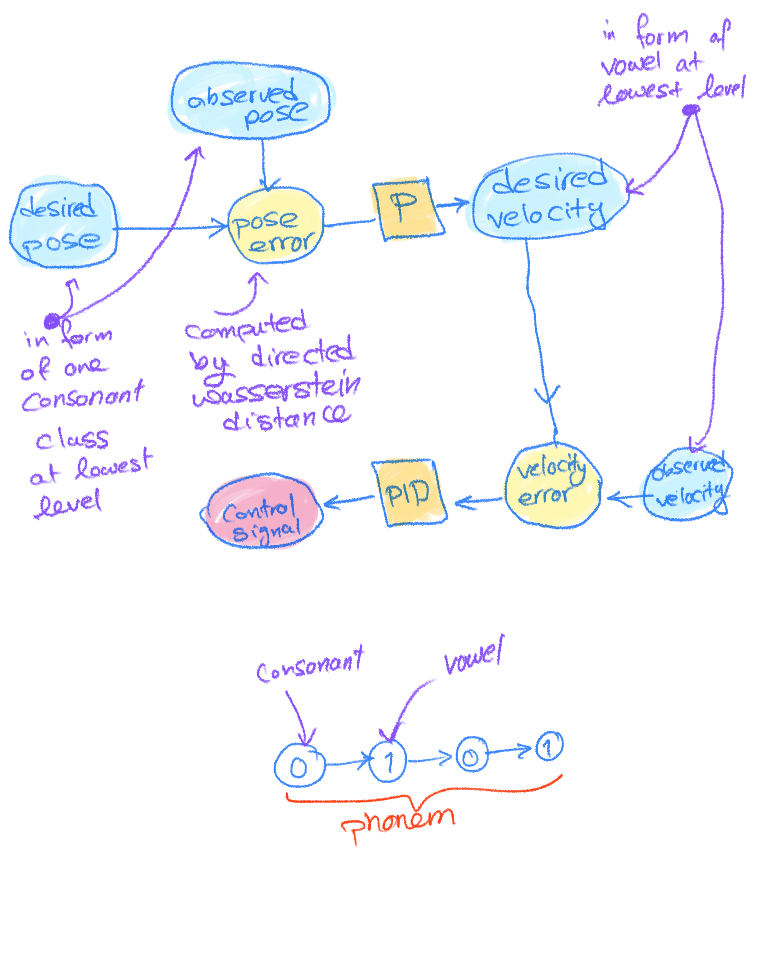
\includegraphics[width=0.9\textwidth]{p_pid_controllers_phonemes_wasserstein.png}
         \end{figure}

         At the physical position level, let \(\mathbf{w}_{p,k}\) denote the directed Wasserstein discrepancy expressed in position coordinates. In the proposed control architecture, it is used as the outer-loop position-error signal,
         \[
         \mathbf{e}^{W}_{p,k}
         =
         \mathbf{w}_{p,k}.
         \]

         A proportional position controller converts this discrepancy into a desired velocity,
         \[
         \mathbf{v}^{\mathrm{sp}}_k
         =
         K_{\mathrm{P},p}\mathbf{e}^{W}_{p,k}
         =
         K_{\mathrm{P},p}\mathbf{w}_{p,k},
         \]
         where \(K_{\mathrm{P},p}\) is the proportional gain of the position loop.

         The velocity tracking error is then
         \[
         \mathbf{e}_{v,k}
         =
         \mathbf{v}^{\mathrm{sp}}_k-\mathbf{v}_k.
         \]

         A PID controller uses this velocity error to generate the low-level control command
         \[
         \mathbf{c}_k
         =
         K_{\mathrm{P},v}\mathbf{e}_{v,k}
         +
         K_{\mathrm{I},v}
         \sum_{j=0}^{k}\mathbf{e}_{v,j}\Delta t
         +
         K_{\mathrm{D},v}
         \frac{\mathbf{e}_{v,k}-\mathbf{e}_{v,k-1}}{\Delta t},
         \]
         where \(K_{\mathrm{P},v}\), \(K_{\mathrm{I},v}\), and \(K_{\mathrm{D},v}\) are the proportional, integral, and derivative gains of the velocity loop.

         Thus, the directed Wasserstein discrepancy provides the direction and magnitude of correction, the outer P controller transforms the position-level discrepancy into a desired velocity, and the inner PID controller drives the system so that the actual velocity follows this desired velocity.

         After the action is executed, a new sensory observation is obtained, the current state distribution is estimated again, and the Wasserstein discrepancy is recomputed. In this way, the perception--action loop is closed and the system continuously reduces discrepancy and surprise.

         \bibliographystyle{plainnat}
         \bibliography{/home/donkarlo/Dropbox/repo/nd_shared_research/bibliography/bibliography.bib}
\end{document}
